\subsection{UC8 - Elaborazione dati}
    \label{uc8}
    
    \begin{figure}[htbp]
        \centering
        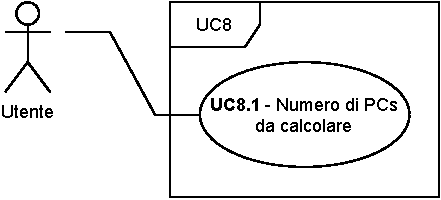
\includegraphics[width=0.5\textwidth]{source/sections/casi-uso/diagrams/uc8.pdf}
        \caption{UC8 - Elaborazione dati}
        \label{fig:uc8}
    \end{figure}
    
    \begin{itemize}
    \item \textbf{Attore}: utente;
    \item \textbf{Descrizione}: vengono elaborati i dati secondo le impostazioni;
    \item \textbf{Precondizione}: 
    \begin{itemize}
        \item eseguito l'upload del dataset come matrice $N\times M$ (\hyperref[uc1]{UC1});
        \item selezionato un tipo di visualizzazione (\hyperref[uc2]{UC2}).
    \end{itemize}  
    \item \textbf{Postcondizione}: l'applicazione dopo che l'utente ha caricato il suo dataset e selezionato il tipo di visualizzazione, ha elaborato i dati secondo le impostazioni;
    \item \textbf{Scenario Principale}: 
    \begin{enumerate}
        \item l'utente carica il suo dataset (\hyperref[uc1]{UC1});
        \item l'utente seleziona il tipo di visualizzazione tra quelle disponibili (\hyperref[uc2]{UC2});
        \item l'applicazione elabora i dati con impostazioni di default (\hyperref[uc8.1]{UC8.1});
        \item l'utente cambia le impostazioni (\hyperref[uc3]{UC3} o \hyperref[uc4]{UC4} o \hyperref[uc5]{UC5} o \hyperref[uc6]{UC6} o \hyperref[uc7]{UC7});
        \item l'applicazione rielabora i dati (\hyperref[uc8.2]{UC8.2}).
    \end{enumerate}
    \end{itemize}
    
    % Nel caso di visualizzazioni che richiedono delle impostazioni obbligatorie? (esempio calcolare matrice di distanza prima di visualizzare il grafico force-field)
    \subsubsection{UC8.1 - Avvio elaborazione dati con impostazioni di default}
    \label{uc8.1}
    \begin{itemize}
    \item \textbf{Attore}: utente;
    \item \textbf{Descrizione}: l'utente avvia l'elaborazione dati secondo le impostazioni di default;
    \item \textbf{Precondizione}: 
    \begin{itemize}
        \item eseguito l'upload del dataset come matrice $N\times M$ (\hyperref[uc1]{UC1});
        \item selezionato un tipo di visualizzazione (\hyperref[uc2]{UC2}).
    \end{itemize}  
    \item \textbf{Postcondizione}: l'applicazione dopo che l'utente ha caricato il suo dataset e selezionato il tipo di visualizzazione, ha avviato l'elaborazione dei dati secondo le impostazioni di default;
    \item \textbf{Scenario Principale}: 
    \begin{enumerate}
        \item l'utente carica il suo dataset (\hyperref[uc1]{UC1});
        \item l'utente seleziona il tipo di visualizzazione tra quelle disponibili (\hyperref[uc2]{UC2});
        \item l'applicazione elabora i dati.
    \end{enumerate}
    \end{itemize}
    
    \subsubsection{UC8.2 - Avvio elaborazione dati con impostazioni utente}
    \label{uc8.2}
    \begin{itemize}
    \item \textbf{Attore}: utente;
    \item \textbf{Descrizione}:  l'utente avvia l'elaborazione dati secondo le impostazioni personalizzate;
    \item \textbf{Precondizione}: 
    \begin{itemize}
        \item eseguito l'upload del dataset come matrice $N\times M$ (\hyperref[uc1]{UC1});
        \item selezionato un tipo di visualizzazione (\hyperref[uc2]{UC2});
        \item l'utente ha cambiato le impostazioni (\hyperref[uc3]{UC3} o \hyperref[uc4]{UC4} o \hyperref[uc5]{UC5} o \hyperref[uc6]{UC6} o \hyperref[uc7]{UC7}).
    \end{itemize}  
    \item \textbf{Postcondizione}: l'applicazione dopo che l'utente ha caricato il suo dataset e selezionato il tipo di visualizzazione, ha avviato l'elaborazione dei dati secondo le impostazioni personalizzate inserite dall'utente;
    \item \textbf{Scenario Principale}: 
    \begin{enumerate}
        \item l'utente carica il suo dataset (\hyperref[uc1]{UC1});
        \item l'utente seleziona il tipo di visualizzazione tra quelle disponibili (\hyperref[uc2]{UC2});
        \item l'applicazione elabora i dati (\hyperref[uc8.1]{UC8.1});
        \item l'utente cambia le impostazioni (\hyperref[uc3]{UC3} o \hyperref[uc4]{UC4} o \hyperref[uc5]{UC5} o \hyperref[uc6]{UC6} o \hyperref[uc7]{UC7});
        \item l'applicazione rielabora i dati.
    \end{enumerate}
    \end{itemize}
